\documentclass{article}
\usepackage{amsmath}
\usepackage{amssymb}
\usepackage{tikz}

\begin{document}

\begin{center}
    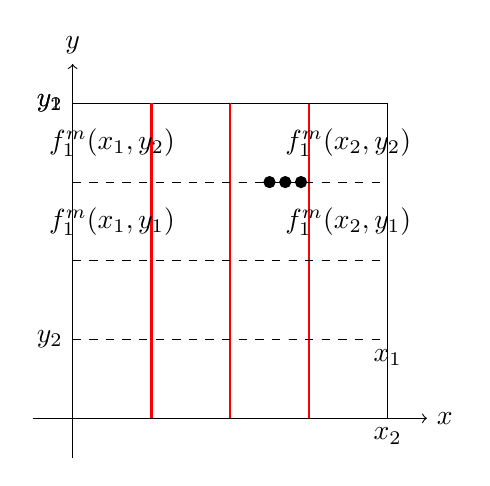
\begin{tikzpicture}[scale=1]
        % Draw axes
        \draw[->] (-0.5,0) -- (4.5,0) node[right] {$x$};
        \draw[->] (0,-0.5) -- (0,4.5) node[above] {$y$};
        
        % Draw grid lines
        \draw[dashed] (0,0) grid (4,4);
        
        % Draw the square boundaries
        \draw (0,0) rectangle (4,4);
        
        % Draw the vertical lines
        \draw[red, thick] (1,0) -- (1,4);
        \draw[red, thick] (2,0) -- (2,4);
        \draw[red, thick] (3,0) -- (3,4);
        
        % Draw the horizontal lines
        \draw[dashed] (0,1) -- (4,1) node[below] {$x_1$};
        \draw[dashed] (0,2) -- (4,2);
        \draw[dashed] (0,3) -- (4,3);
        \draw[dashed] (0,4) node[left] {$y_1$} -- (4,4);
        \draw[dashed] (0,0) -- (4,0) node[below] {$x_2$};
        \draw[dashed] (0,1) node[left] {$y_2$} -- (4,1);
        \draw[dashed] (0,2) -- (4,2);
        \draw[dashed] (0,3) -- (4,3);
        \draw[dashed] (0,4) node[left] {$y_2$} -- (4,4);
        
        % Label the functions
        \node at (0.5, 3.5) {$f_{1}^{m}(x_1, y_2)$};
        \node at (0.5, 2.5) {$f_{1}^{m}(x_1, y_1)$};
        \node at (3.5, 3.5) {$f_{1}^{m}(x_2, y_2)$};
        \node at (3.5, 2.5) {$f_{1}^{m}(x_2, y_1)$};
        
        % Draw the dots
        \filldraw[black] (2.5, 3) circle (2pt);
        \filldraw[black] (2.7, 3) circle (2pt);
        \filldraw[black] (2.9, 3) circle (2pt);
    \end{tikzpicture}
\end{center}

For some \( m \in \mathbb{N} \), the action of \( f^m \) on the square bounded by \( x = x_1 \), \( x = x_2 \), \( y = y_1 \) and \( y = y_2 \) determined by the red region.

\end{document}